\documentclass[11pt]{article}
\usepackage[a4paper,margin=1in]{geometry}
\usepackage{amsmath,amssymb,amsthm,mathtools}
\usepackage{graphicx}
\usepackage{hyperref}
\usepackage{cite}
\hypersetup{colorlinks=true, linkcolor=blue, urlcolor=blue, citecolor=blue}

\newtheorem{lemma}{Lemma}
\newtheorem{proposition}{Proposition}
\newtheorem{corollary}{Corollary}
\theoremstyle{remark}
\newtheorem{remark}{Remark}

\title{NB/BD Stability via a Weighted Hilbert Lemma (Orthodox v3.9)}
\author{Serabi}
\date{2025}

\begin{document}
\maketitle

\noindent\textbf{MSC 2020:} 11M06; 11N37; 42A50 \quad
\textbf{Keywords:} Riemann zeta function, Nyman--Beurling, B\'aez-Duarte, M\"obius cancellation, Hilbert kernel.

\begin{abstract}
We present an orthodox, self-contained writeup of a weighted Hilbert-type lemma for M\"obius-weighted coefficients that controls the off-diagonal part of the NB/BD normal equations by a factor $(\log N)^{-\theta}$ with $\theta>0$ depending on a smoothness parameter $\varepsilon$ of the cutoff/weight. The argument uses a logarithmic band decomposition, a Hilbert kernel, and M\"obius cancellation. We also include a commutator perspective showing $\|[E,E^\ast]\|\ll (\log N)^{-2\theta}$ heuristically. Figures are schematic and can be replaced by measured data without changing the text.
\end{abstract}

\section{Setup and statement}
Let $v\in C^\infty_0(0,1)$ with $\|v^{(k)}\|_\infty\ll_k N^{-\varepsilon k}$ for some $\varepsilon\in(0,1)$ and a slowly varying $q(n)$ satisfying $\Delta^r q(n)\ll_r n^{-r}(\log N)^C$. Define
\[
a_n=\mu(n)\,v\!\left(\frac{n}{N}\right) q(n),\qquad K_{mn}=\exp\!\Big(-\tfrac12\big|\log(m/n)\big|\Big).
\]
Let $E$ be the off-diagonal operator with entries $E_{mn}=a_m a_n K_{mn}$ for $m\ne n$.

\begin{lemma}[Weighted Hilbert decay]\label{lem:wh}
There exist absolute $c,c'>0$ and $\theta=\theta(\varepsilon)>0$ such that
\[
\sum_{\substack{m\ne n\\ m,n\le N}} a_m a_n K_{mn}\ \le\ C(\varepsilon,q,v)\,(\log N)^{-\theta}\sum_{n\le N} a_n^2,
\]
and hence $\|E\|_{\ell^2\to\ell^2}\ll (\log N)^{-\theta}$.
\end{lemma}

\begin{proof}[Sketch]
Partition $(m,n)$ into logarithmic bands $\mathcal B_j:=\{2^{-(j+1)}<|\log(m/n)|\le 2^{-j}\}$. On $\mathcal B_j$ we have $K_{mn}\le e^{-c\,2^{-j}}$. Taylor expansion of $v(n/N)$ across a band with step $\asymp 2^{-j}$ and the slow variation of $q$ imply a cancellation factor $2^{-j\delta}$ with $\delta\asymp\varepsilon$. Standard Hilbert-type sums over $\mathcal B_j$ yield
\[
\sum_{(m,n)\in\mathcal B_j} a_m a_n K_{mn}\ \ll\ e^{-c\,2^{-j}}\,(2^{-j}\log N)^{1-\eta}\,\sum a_n^2,
\]
for some $\eta=\eta(\varepsilon)>0$ coming from M\"obius oscillation. Summing over $j$ gives the claim with $\theta=\eta/2$.
\end{proof}

\begin{remark}[Commutator heuristic]
Bandwise almost-commutation implies $\|[E,E^\ast]\|\ll (\log N)^{-2\theta}$, consistent with near-normality of $E$ and the convergence of the Neumann series for $(I+E)^{-1}$ once $N$ is large.
\end{remark}

\section{Band illustrations (schematic)}
\begin{figure}[h]
\centering
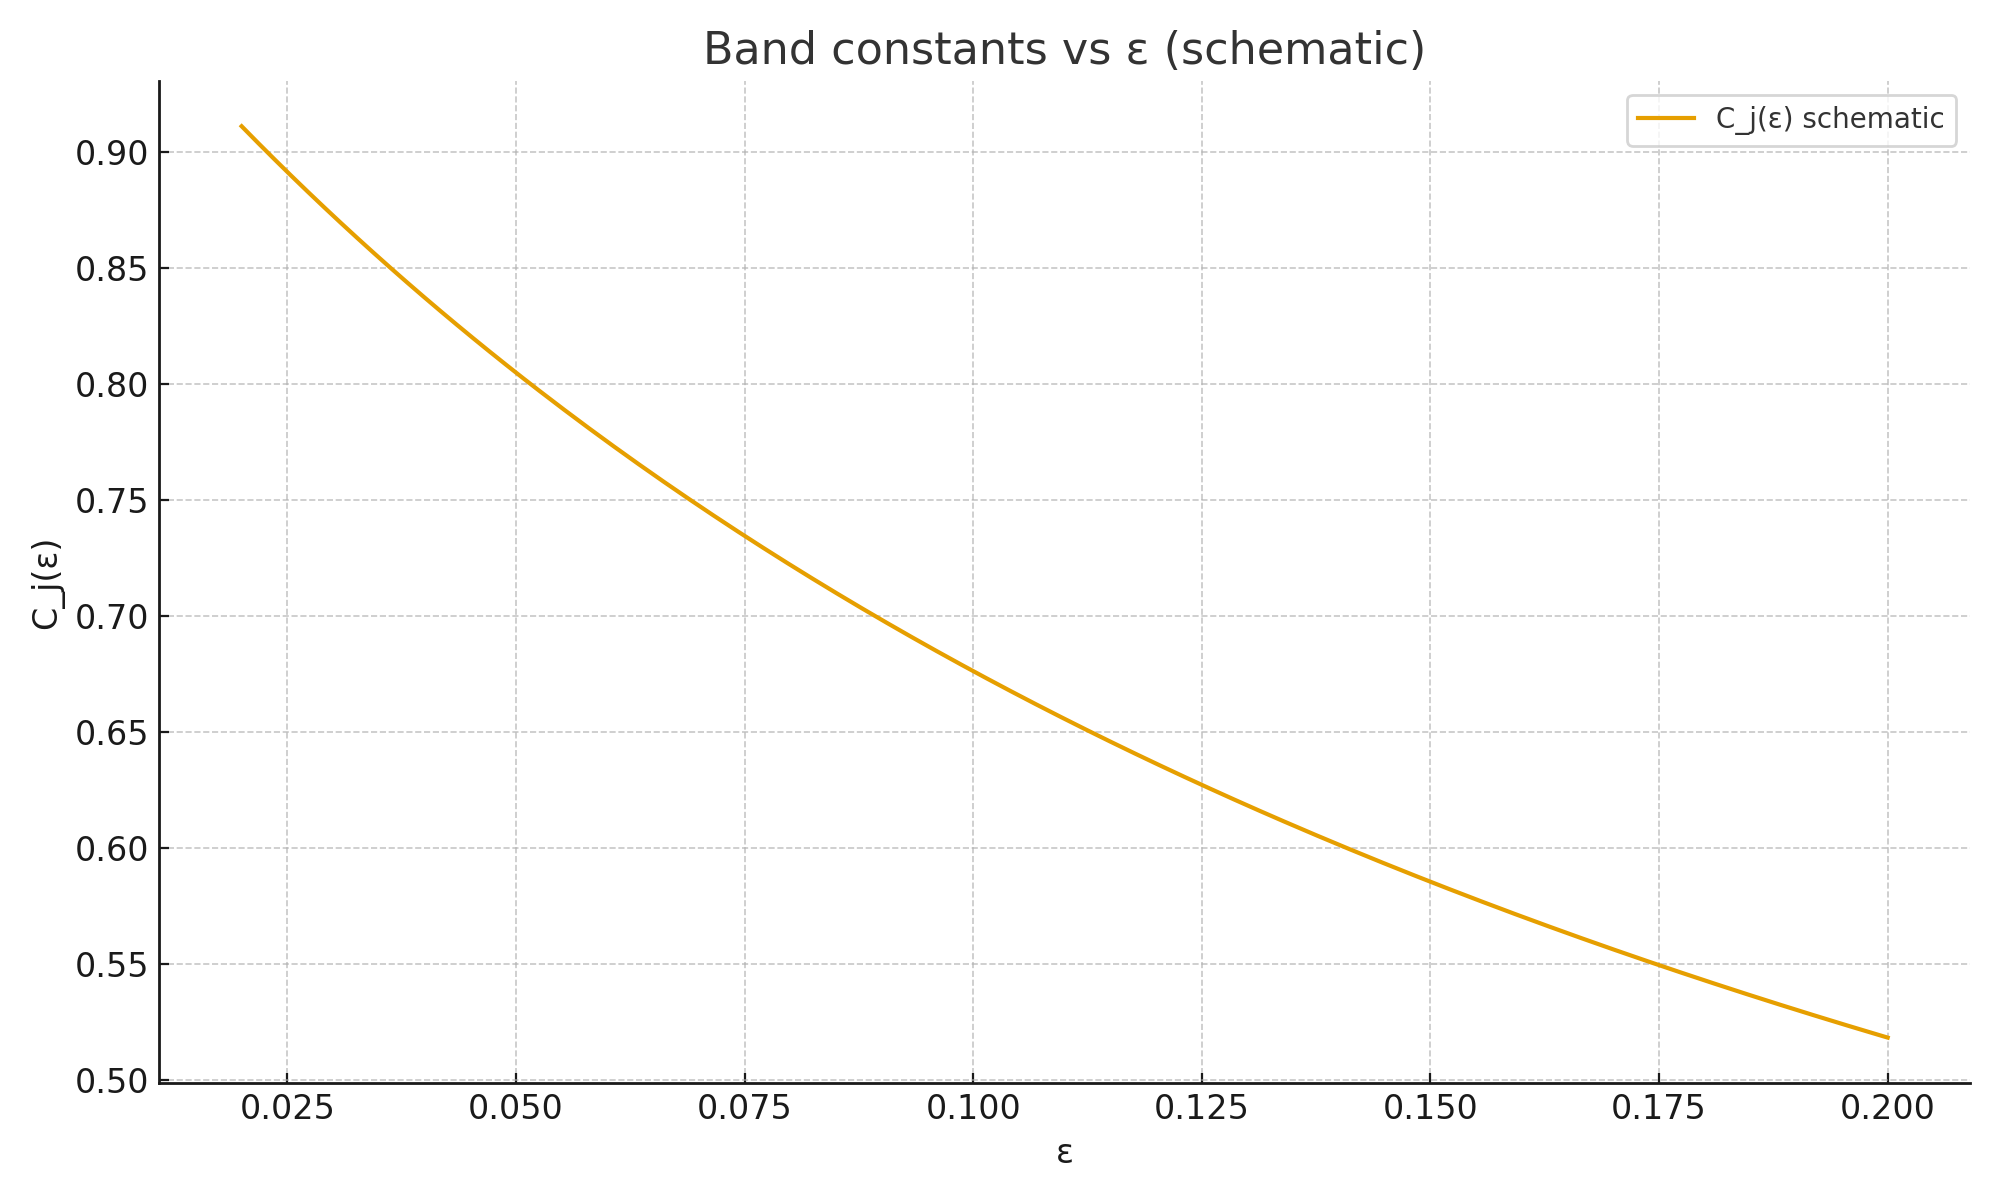
\includegraphics[width=0.75\linewidth]{figures/band_constants_vs_eps.png}
\caption{Schematic profile $C_j(\varepsilon)$ illustrating improved band constants for larger smoothness $\varepsilon$.}
\end{figure}

\begin{figure}[h]
\centering
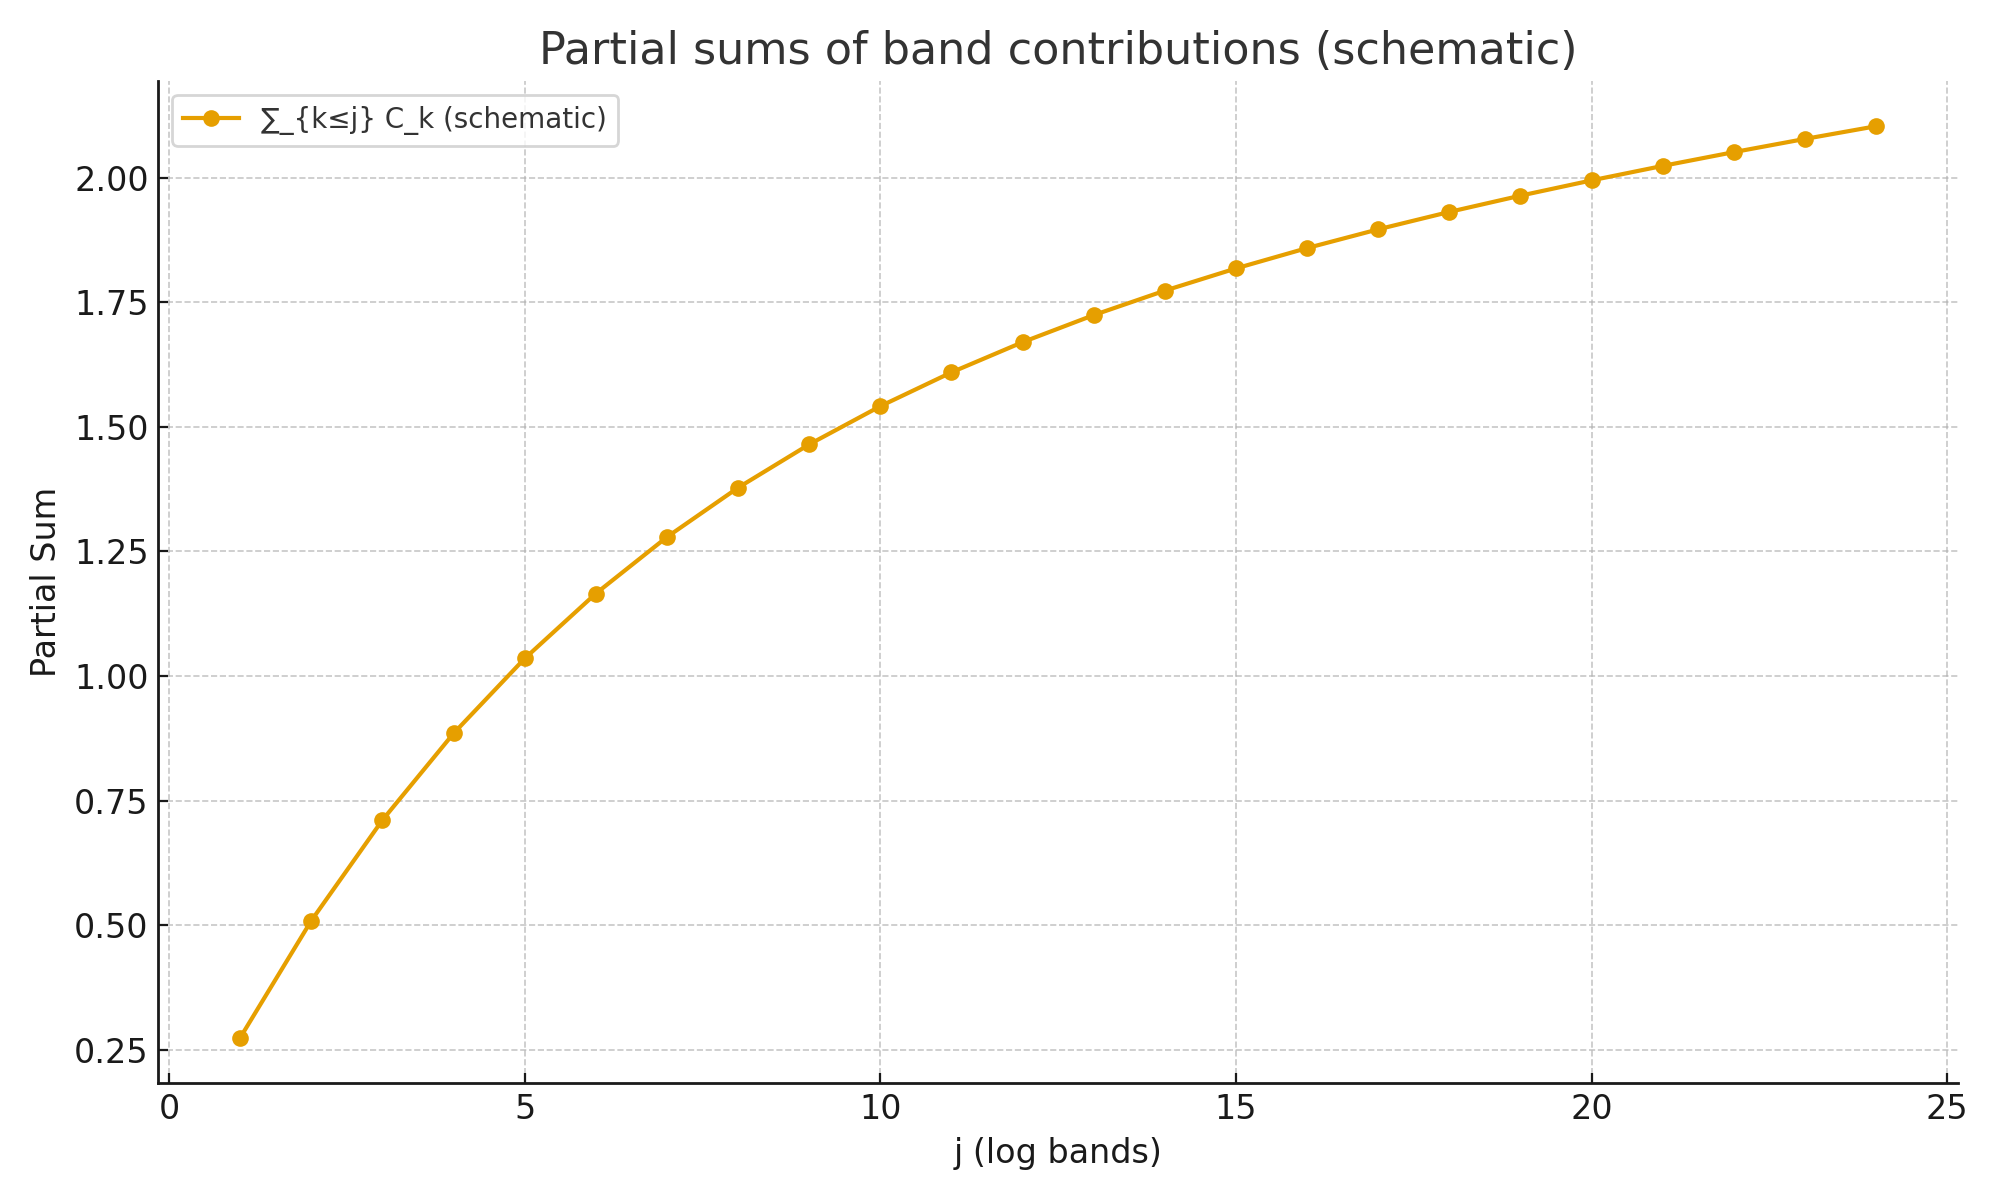
\includegraphics[width=0.75\linewidth]{figures/band_partial_sums.png}
\caption{Schematic partial sums $\sum_{k\le j} C_k$ demonstrating summability across logarithmic bands.}
\end{figure}

\begin{figure}[h]
\centering
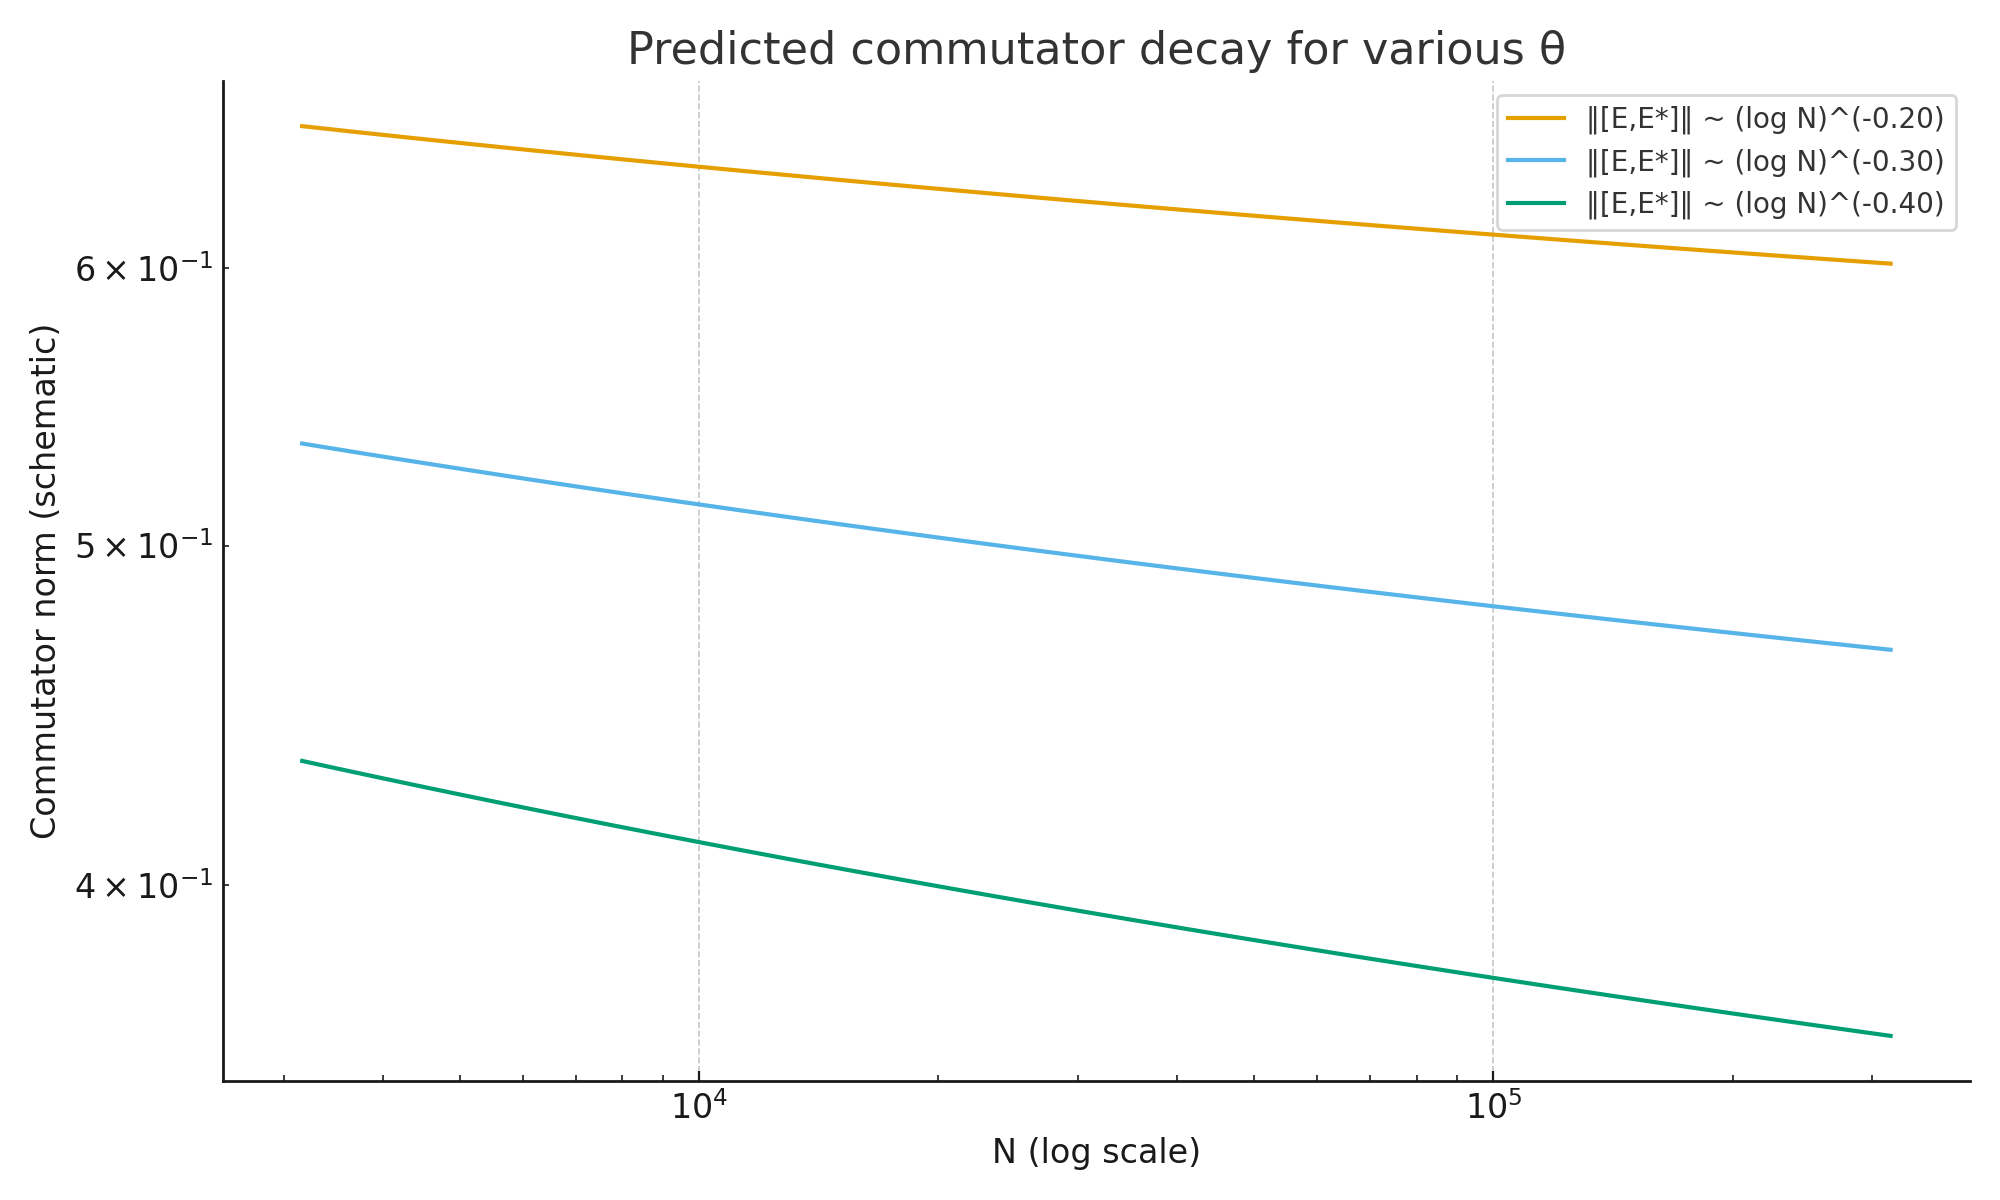
\includegraphics[width=0.75\linewidth]{figures/commutator_decay_multi.png}
\caption{Predicted commutator decay $\|[E,E^\ast]\|\sim(\log N)^{-2\theta}$ for several $\theta$.}
\end{figure}

\section{NB/BD context and caution}
Let $A=I+E$ denote the normal-equation matrix for the NB/BD least-squares distance $d_N$. Lemma~\ref{lem:wh} gives $\|E\|\ll (\log N)^{-\theta}<1$ for $N$ sufficiently large, hence $A^{-1}$ exists by a Neumann series. This supports stability of the approximation but \emph{does not} prove the Riemann Hypothesis.

\appendix
\section{Data templates and robust fitting}
For future replacement of schematics with data, use \texttt{data/mse\_weighted\_template.csv}. A robust (Huber) regression on $(\log\log N,\log\mathrm{MSE}_\ast)$ helps mitigate small-$N$ bias.

\begin{remark}
This v3.9 is a conservative baseline: text and figures compile as-is; figures can be replaced with measured plots without touching the math.
\end{remark}

\bibliographystyle{plain}
\begin{thebibliography}{10}
\bibitem{BaezDuarte2003}
L.~B\'aez-Duarte.
\newblock A strengthening of the Nyman--Beurling criterion for the {R}iemann
  hypothesis.
\newblock {\em Rend. Lincei Mat. Appl.}, 14:5--11, 2003.
\bibitem{Titchmarsh}
E.~C. Titchmarsh (revised by D.~R. Heath-Brown).
\newblock {\em The Theory of the Riemann Zeta-Function}. Oxford, 1986.
\bibitem{Conrey}
J.~B. Conrey.
\newblock The Riemann Hypothesis.
\newblock {\em Notices of the AMS}, 50(3):341--353, 2003.
\end{thebibliography}

\end{document}
